\documentclass[twoside]{book}

% Packages required by doxygen
\usepackage{fixltx2e}
\usepackage{calc}
\usepackage{doxygen}
\usepackage[export]{adjustbox} % also loads graphicx
\usepackage{graphicx}
\usepackage[utf8]{inputenc}
\usepackage{makeidx}
\usepackage{multicol}
\usepackage{multirow}
\PassOptionsToPackage{warn}{textcomp}
\usepackage{textcomp}
\usepackage[nointegrals]{wasysym}
\usepackage[table]{xcolor}

% Font selection
\usepackage[T1]{fontenc}
\usepackage[scaled=.90]{helvet}
\usepackage{courier}
\usepackage{amssymb}
\usepackage{sectsty}
\renewcommand{\familydefault}{\sfdefault}
\allsectionsfont{%
  \fontseries{bc}\selectfont%
  \color{darkgray}%
}
\renewcommand{\DoxyLabelFont}{%
  \fontseries{bc}\selectfont%
  \color{darkgray}%
}
\newcommand{\+}{\discretionary{\mbox{\scriptsize$\hookleftarrow$}}{}{}}

% Page & text layout
\usepackage{geometry}
\geometry{%
  a4paper,%
  top=2.5cm,%
  bottom=2.5cm,%
  left=2.5cm,%
  right=2.5cm%
}
\tolerance=750
\hfuzz=15pt
\hbadness=750
\setlength{\emergencystretch}{15pt}
\setlength{\parindent}{0cm}
\setlength{\parskip}{3ex plus 2ex minus 2ex}
\makeatletter
\renewcommand{\paragraph}{%
  \@startsection{paragraph}{4}{0ex}{-1.0ex}{1.0ex}{%
    \normalfont\normalsize\bfseries\SS@parafont%
  }%
}
\renewcommand{\subparagraph}{%
  \@startsection{subparagraph}{5}{0ex}{-1.0ex}{1.0ex}{%
    \normalfont\normalsize\bfseries\SS@subparafont%
  }%
}
\makeatother

% Headers & footers
\usepackage{fancyhdr}
\pagestyle{fancyplain}
\fancyhead[LE]{\fancyplain{}{\bfseries\thepage}}
\fancyhead[CE]{\fancyplain{}{}}
\fancyhead[RE]{\fancyplain{}{\bfseries\leftmark}}
\fancyhead[LO]{\fancyplain{}{\bfseries\rightmark}}
\fancyhead[CO]{\fancyplain{}{}}
\fancyhead[RO]{\fancyplain{}{\bfseries\thepage}}
\fancyfoot[LE]{\fancyplain{}{}}
\fancyfoot[CE]{\fancyplain{}{}}
\fancyfoot[RE]{\fancyplain{}{\bfseries\scriptsize Generated by Doxygen }}
\fancyfoot[LO]{\fancyplain{}{\bfseries\scriptsize Generated by Doxygen }}
\fancyfoot[CO]{\fancyplain{}{}}
\fancyfoot[RO]{\fancyplain{}{}}
\renewcommand{\footrulewidth}{0.4pt}
\renewcommand{\chaptermark}[1]{%
  \markboth{#1}{}%
}
\renewcommand{\sectionmark}[1]{%
  \markright{\thesection\ #1}%
}

% Indices & bibliography
\usepackage{natbib}
\usepackage[titles]{tocloft}
\setcounter{tocdepth}{3}
\setcounter{secnumdepth}{5}
\makeindex

% Hyperlinks (required, but should be loaded last)
\usepackage{ifpdf}
\ifpdf
  \usepackage[pdftex,pagebackref=true]{hyperref}
\else
  \usepackage[ps2pdf,pagebackref=true]{hyperref}
\fi
\hypersetup{%
  colorlinks=true,%
  linkcolor=blue,%
  citecolor=blue,%
  unicode%
}

% Custom commands
\newcommand{\clearemptydoublepage}{%
  \newpage{\pagestyle{empty}\cleardoublepage}%
}

\usepackage{caption}
\captionsetup{labelsep=space,justification=centering,font={bf},singlelinecheck=off,skip=4pt,position=top}

%===== C O N T E N T S =====

\begin{document}

% Titlepage & ToC
\hypersetup{pageanchor=false,
             bookmarksnumbered=true,
             pdfencoding=unicode
            }
\pagenumbering{roman}
\begin{titlepage}
\vspace*{7cm}
\begin{center}%
{\Large G\+A\+ME }\\
\vspace*{1cm}
{\large Generated by Doxygen 1.8.11}\\
\end{center}
\end{titlepage}
\clearemptydoublepage
\tableofcontents
\clearemptydoublepage
\pagenumbering{arabic}
\hypersetup{pageanchor=true}

%--- Begin generated contents ---
\chapter{Class Index}
\section{Data Structures}
Here are the data structures with brief descriptions\+:\begin{DoxyCompactList}
\item\contentsline{section}{\hyperlink{structbackground}{background} }{\pageref{structbackground}}{}
\item\contentsline{section}{\hyperlink{structennemi}{ennemi} }{\pageref{structennemi}}{}
\item\contentsline{section}{\hyperlink{structpersonnage}{personnage} }{\pageref{structpersonnage}}{}
\item\contentsline{section}{\hyperlink{structscore}{score} }{\pageref{structscore}}{}
\item\contentsline{section}{\hyperlink{structtimer}{timer} }{\pageref{structtimer}}{}
\item\contentsline{section}{\hyperlink{structvie}{vie} }{\pageref{structvie}}{}
\end{DoxyCompactList}

\chapter{File Index}
\section{File List}
Here is a list of all files with brief descriptions\+:\begin{DoxyCompactList}
\item\contentsline{section}{\hyperlink{main_8c}{main.\+c} }{\pageref{main_8c}}{}
\item\contentsline{section}{\hyperlink{perso_8c}{perso.\+c} }{\pageref{perso_8c}}{}
\item\contentsline{section}{\hyperlink{perso_8h}{perso.\+h} }{\pageref{perso_8h}}{}
\end{DoxyCompactList}

\chapter{Class Documentation}
\hypertarget{structbackground}{}\section{background Struct Reference}
\label{structbackground}\index{background@{background}}


struct for background  




{\ttfamily \#include $<$save.\+h$>$}

\subsection*{Public Attributes}
\begin{DoxyCompactItemize}
\item 
S\+D\+L\+\_\+\+Surface $\ast$ \hyperlink{structbackground_a1c5c3a3ebb56924b9f829602f9641006}{img}
\item 
S\+D\+L\+\_\+\+Rect \hyperlink{structbackground_aa70f1467505f43c50fec228c21bd7af4}{pos}
\end{DoxyCompactItemize}


\subsection{Detailed Description}
struct for background 

\subsection{Member Data Documentation}
\index{background@{background}!img@{img}}
\index{img@{img}!background@{background}}
\subsubsection[{\texorpdfstring{img}{img}}]{\setlength{\rightskip}{0pt plus 5cm}S\+D\+L\+\_\+\+Surface$\ast$ background\+::img}\hypertarget{structbackground_a1c5c3a3ebb56924b9f829602f9641006}{}\label{structbackground_a1c5c3a3ebb56924b9f829602f9641006}
\index{background@{background}!pos@{pos}}
\index{pos@{pos}!background@{background}}
\subsubsection[{\texorpdfstring{pos}{pos}}]{\setlength{\rightskip}{0pt plus 5cm}S\+D\+L\+\_\+\+Rect background\+::pos}\hypertarget{structbackground_aa70f1467505f43c50fec228c21bd7af4}{}\label{structbackground_aa70f1467505f43c50fec228c21bd7af4}


The documentation for this struct was generated from the following file\+:\begin{DoxyCompactItemize}
\item 
\hyperlink{save_8h}{save.\+h}\end{DoxyCompactItemize}

\hypertarget{structpersonnage}{}\section{personnage Struct Reference}
\label{structpersonnage}\index{personnage@{personnage}}


{\ttfamily \#include $<$struct.\+h$>$}



Collaboration diagram for personnage\+:
\nopagebreak
\begin{figure}[H]
\begin{center}
\leavevmode
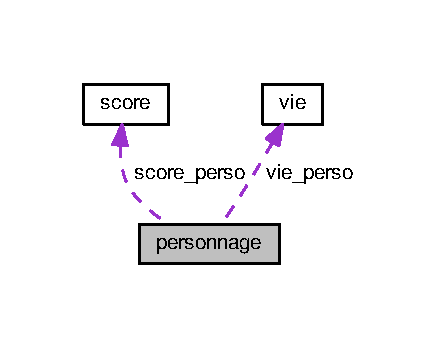
\includegraphics[width=211pt]{structpersonnage__coll__graph}
\end{center}
\end{figure}
\subsection*{Data Fields}
\begin{DoxyCompactItemize}
\item 
S\+D\+L\+\_\+\+Surface $\ast$ \hyperlink{structpersonnage_a3fc8b5a6848cc4b09b844f482411a414}{sprite} \mbox{[}12\mbox{]}
\item 
S\+D\+L\+\_\+\+Rect \hyperlink{structpersonnage_a4a45c9e4310d819fcd3c9a60fc8c0ebf}{position\+\_\+perso}
\item 
int \hyperlink{structpersonnage_a2664acffa6fccd8487b9e03b63fbd6da}{direction}
\item 
\hyperlink{structvie}{vie} \hyperlink{structpersonnage_ac96f4aee44111bc31a7718e5762bf483}{vie\+\_\+perso}
\item 
\hyperlink{structscore}{score} \hyperlink{structpersonnage_a7ea99b7d0c8445cb3d7ba6717eb89d8c}{score\+\_\+perso}
\item 
int \hyperlink{structpersonnage_acfac32928075716cc10265cfc9f551fc}{num}
\end{DoxyCompactItemize}


\subsection{Field Documentation}
\mbox{\Hypertarget{structpersonnage_a2664acffa6fccd8487b9e03b63fbd6da}\label{structpersonnage_a2664acffa6fccd8487b9e03b63fbd6da}} 
\index{personnage@{personnage}!direction@{direction}}
\index{direction@{direction}!personnage@{personnage}}
\subsubsection{\texorpdfstring{direction}{direction}}
{\footnotesize\ttfamily int personnage\+::direction}

\mbox{\Hypertarget{structpersonnage_acfac32928075716cc10265cfc9f551fc}\label{structpersonnage_acfac32928075716cc10265cfc9f551fc}} 
\index{personnage@{personnage}!num@{num}}
\index{num@{num}!personnage@{personnage}}
\subsubsection{\texorpdfstring{num}{num}}
{\footnotesize\ttfamily int personnage\+::num}

\mbox{\Hypertarget{structpersonnage_a4a45c9e4310d819fcd3c9a60fc8c0ebf}\label{structpersonnage_a4a45c9e4310d819fcd3c9a60fc8c0ebf}} 
\index{personnage@{personnage}!position\+\_\+perso@{position\+\_\+perso}}
\index{position\+\_\+perso@{position\+\_\+perso}!personnage@{personnage}}
\subsubsection{\texorpdfstring{position\+\_\+perso}{position\_perso}}
{\footnotesize\ttfamily S\+D\+L\+\_\+\+Rect personnage\+::position\+\_\+perso}

\mbox{\Hypertarget{structpersonnage_a7ea99b7d0c8445cb3d7ba6717eb89d8c}\label{structpersonnage_a7ea99b7d0c8445cb3d7ba6717eb89d8c}} 
\index{personnage@{personnage}!score\+\_\+perso@{score\+\_\+perso}}
\index{score\+\_\+perso@{score\+\_\+perso}!personnage@{personnage}}
\subsubsection{\texorpdfstring{score\+\_\+perso}{score\_perso}}
{\footnotesize\ttfamily \hyperlink{structscore}{score} personnage\+::score\+\_\+perso}

\mbox{\Hypertarget{structpersonnage_a3fc8b5a6848cc4b09b844f482411a414}\label{structpersonnage_a3fc8b5a6848cc4b09b844f482411a414}} 
\index{personnage@{personnage}!sprite@{sprite}}
\index{sprite@{sprite}!personnage@{personnage}}
\subsubsection{\texorpdfstring{sprite}{sprite}}
{\footnotesize\ttfamily S\+D\+L\+\_\+\+Surface$\ast$ personnage\+::sprite\mbox{[}12\mbox{]}}

\mbox{\Hypertarget{structpersonnage_ac96f4aee44111bc31a7718e5762bf483}\label{structpersonnage_ac96f4aee44111bc31a7718e5762bf483}} 
\index{personnage@{personnage}!vie\+\_\+perso@{vie\+\_\+perso}}
\index{vie\+\_\+perso@{vie\+\_\+perso}!personnage@{personnage}}
\subsubsection{\texorpdfstring{vie\+\_\+perso}{vie\_perso}}
{\footnotesize\ttfamily \hyperlink{structvie}{vie} personnage\+::vie\+\_\+perso}



The documentation for this struct was generated from the following file\+:\begin{DoxyCompactItemize}
\item 
\hyperlink{struct_8h}{struct.\+h}\end{DoxyCompactItemize}

\hypertarget{structscore}{}\section{score Struct Reference}
\label{structscore}\index{score@{score}}


struct for score of hero  




{\ttfamily \#include $<$perso.\+h$>$}

\subsection*{Public Attributes}
\begin{DoxyCompactItemize}
\item 
int \hyperlink{structscore_a86ee1f22a5bf4e92781f2b2165aa0859}{score\+\_\+atteint}
\item 
S\+D\+L\+\_\+\+Rect \hyperlink{structscore_a444e826e64d1abf14dc0108095752cc1}{position\+\_\+score}
\item 
T\+T\+F\+\_\+\+Font $\ast$ \hyperlink{structscore_aa8088c00f0a0ce91db39deb03afc7110}{police\+\_\+score}
\item 
S\+D\+L\+\_\+\+Surface $\ast$ \hyperlink{structscore_aa5918332d1797da4bedaccfce5446b88}{score\+\_\+texte}
\end{DoxyCompactItemize}


\subsection{Detailed Description}
struct for score of hero 

\subsection{Member Data Documentation}
\index{score@{score}!police\+\_\+score@{police\+\_\+score}}
\index{police\+\_\+score@{police\+\_\+score}!score@{score}}
\subsubsection[{\texorpdfstring{police\+\_\+score}{police_score}}]{\setlength{\rightskip}{0pt plus 5cm}T\+T\+F\+\_\+\+Font$\ast$ score\+::police\+\_\+score}\hypertarget{structscore_aa8088c00f0a0ce91db39deb03afc7110}{}\label{structscore_aa8088c00f0a0ce91db39deb03afc7110}
font \index{score@{score}!position\+\_\+score@{position\+\_\+score}}
\index{position\+\_\+score@{position\+\_\+score}!score@{score}}
\subsubsection[{\texorpdfstring{position\+\_\+score}{position_score}}]{\setlength{\rightskip}{0pt plus 5cm}S\+D\+L\+\_\+\+Rect score\+::position\+\_\+score}\hypertarget{structscore_a444e826e64d1abf14dc0108095752cc1}{}\label{structscore_a444e826e64d1abf14dc0108095752cc1}
rectangle \index{score@{score}!score\+\_\+atteint@{score\+\_\+atteint}}
\index{score\+\_\+atteint@{score\+\_\+atteint}!score@{score}}
\subsubsection[{\texorpdfstring{score\+\_\+atteint}{score_atteint}}]{\setlength{\rightskip}{0pt plus 5cm}int score\+::score\+\_\+atteint}\hypertarget{structscore_a86ee1f22a5bf4e92781f2b2165aa0859}{}\label{structscore_a86ee1f22a5bf4e92781f2b2165aa0859}
entier \index{score@{score}!score\+\_\+texte@{score\+\_\+texte}}
\index{score\+\_\+texte@{score\+\_\+texte}!score@{score}}
\subsubsection[{\texorpdfstring{score\+\_\+texte}{score_texte}}]{\setlength{\rightskip}{0pt plus 5cm}S\+D\+L\+\_\+\+Surface$\ast$ score\+::score\+\_\+texte}\hypertarget{structscore_aa5918332d1797da4bedaccfce5446b88}{}\label{structscore_aa5918332d1797da4bedaccfce5446b88}
surface 

The documentation for this struct was generated from the following file\+:\begin{DoxyCompactItemize}
\item 
\hyperlink{perso_8h}{perso.\+h}\end{DoxyCompactItemize}

\hypertarget{structvie}{}\section{vie Struct Reference}
\label{structvie}\index{vie@{vie}}


struct for vie perso  




{\ttfamily \#include $<$save.\+h$>$}

\subsection*{Public Attributes}
\begin{DoxyCompactItemize}
\item 
int \hyperlink{structvie_ace0f84a19ce4f5854ec56c137b33b947}{nbredevie}
\item 
S\+D\+L\+\_\+\+Surface $\ast$ \hyperlink{structvie_a2c29f60898de16e1306bd1043fa38dc9}{vie} \mbox{[}4\mbox{]}
\item 
S\+D\+L\+\_\+\+Rect \hyperlink{structvie_aaa37f269f7261984f2e540534210af5a}{position\+\_\+de\+\_\+vie}
\end{DoxyCompactItemize}


\subsection{Detailed Description}
struct for vie perso 

\subsection{Member Data Documentation}
\index{vie@{vie}!nbredevie@{nbredevie}}
\index{nbredevie@{nbredevie}!vie@{vie}}
\subsubsection[{\texorpdfstring{nbredevie}{nbredevie}}]{\setlength{\rightskip}{0pt plus 5cm}int vie\+::nbredevie}\hypertarget{structvie_ace0f84a19ce4f5854ec56c137b33b947}{}\label{structvie_ace0f84a19ce4f5854ec56c137b33b947}
entier \index{vie@{vie}!position\+\_\+de\+\_\+vie@{position\+\_\+de\+\_\+vie}}
\index{position\+\_\+de\+\_\+vie@{position\+\_\+de\+\_\+vie}!vie@{vie}}
\subsubsection[{\texorpdfstring{position\+\_\+de\+\_\+vie}{position_de_vie}}]{\setlength{\rightskip}{0pt plus 5cm}S\+D\+L\+\_\+\+Rect vie\+::position\+\_\+de\+\_\+vie}\hypertarget{structvie_aaa37f269f7261984f2e540534210af5a}{}\label{structvie_aaa37f269f7261984f2e540534210af5a}
rectangle \index{vie@{vie}!vie@{vie}}
\index{vie@{vie}!vie@{vie}}
\subsubsection[{\texorpdfstring{vie}{vie}}]{\setlength{\rightskip}{0pt plus 5cm}S\+D\+L\+\_\+\+Surface$\ast$ vie\+::vie\mbox{[}4\mbox{]}}\hypertarget{structvie_a2c29f60898de16e1306bd1043fa38dc9}{}\label{structvie_a2c29f60898de16e1306bd1043fa38dc9}
surface 

The documentation for this struct was generated from the following file\+:\begin{DoxyCompactItemize}
\item 
\hyperlink{save_8h}{save.\+h}\end{DoxyCompactItemize}

\chapter{File Documentation}
\hypertarget{main_8c}{}\section{main.\+c File Reference}
\label{main_8c}\index{main.\+c@{main.\+c}}
{\ttfamily \#include $<$stdio.\+h$>$}\newline
{\ttfamily \#include $<$stdlib.\+h$>$}\newline
{\ttfamily \#include $<$S\+D\+L/\+S\+D\+L.\+h$>$}\newline
{\ttfamily \#include $<$S\+D\+L/\+S\+D\+L\+\_\+image.\+h$>$}\newline
{\ttfamily \#include $<$S\+D\+L/\+S\+D\+L\+\_\+ttf.\+h$>$}\newline
{\ttfamily \#include \char`\"{}S\+D\+L/\+S\+D\+L\+\_\+mixer.\+h\char`\"{}}\newline
{\ttfamily \#include \char`\"{}menu.\+h\char`\"{}}\newline
Include dependency graph for main.\+c\+:
\nopagebreak
\begin{figure}[H]
\begin{center}
\leavevmode
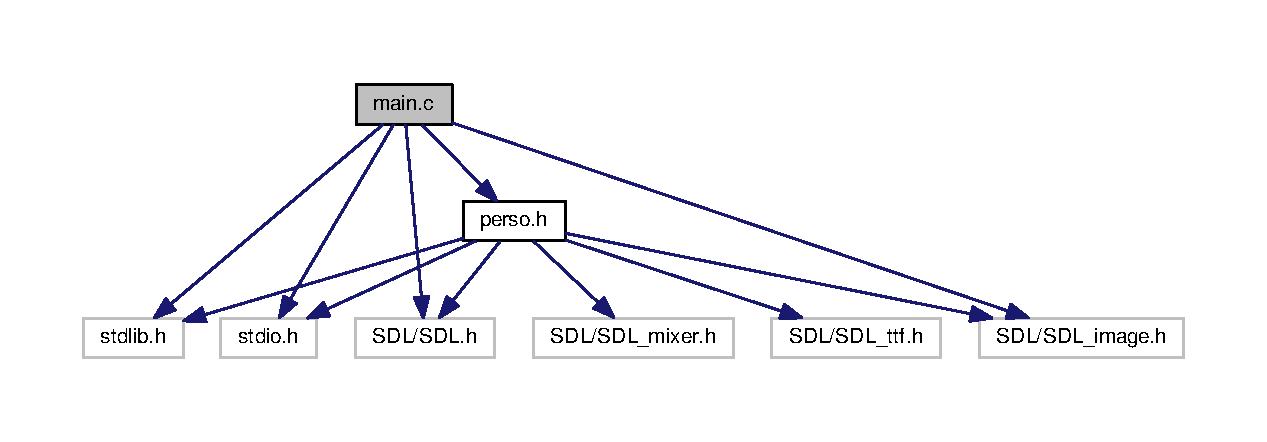
\includegraphics[width=350pt]{main_8c__incl}
\end{center}
\end{figure}
\subsection*{Functions}
\begin{DoxyCompactItemize}
\item 
int \hyperlink{main_8c_ae66f6b31b5ad750f1fe042a706a4e3d4}{main} ()
\end{DoxyCompactItemize}


\subsection{Function Documentation}
\mbox{\Hypertarget{main_8c_ae66f6b31b5ad750f1fe042a706a4e3d4}\label{main_8c_ae66f6b31b5ad750f1fe042a706a4e3d4}} 
\index{main.\+c@{main.\+c}!main@{main}}
\index{main@{main}!main.\+c@{main.\+c}}
\subsubsection{\texorpdfstring{main()}{main()}}
{\footnotesize\ttfamily int main (\begin{DoxyParamCaption}{ }\end{DoxyParamCaption})}

Here is the call graph for this function\+:
\nopagebreak
\begin{figure}[H]
\begin{center}
\leavevmode
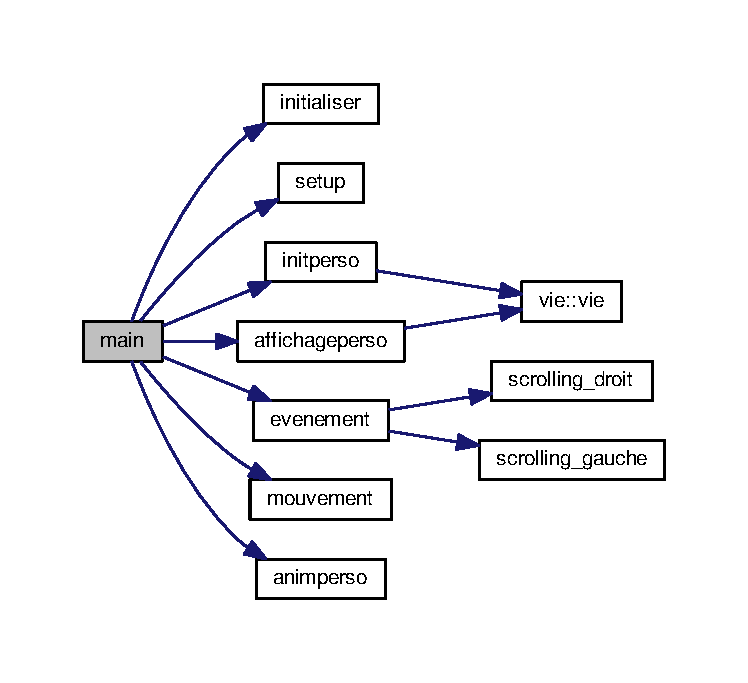
\includegraphics[width=350pt]{main_8c_ae66f6b31b5ad750f1fe042a706a4e3d4_cgraph}
\end{center}
\end{figure}

\hypertarget{perso_8c}{}\section{perso.\+c File Reference}
\label{perso_8c}\index{perso.\+c@{perso.\+c}}
{\ttfamily \#include \char`\"{}perso.\+h\char`\"{}}\\*
{\ttfamily \#include $<$stdio.\+h$>$}\\*
{\ttfamily \#include $<$stdlib.\+h$>$}\\*
{\ttfamily \#include \char`\"{}S\+D\+L/\+S\+D\+L.\+h\char`\"{}}\\*
{\ttfamily \#include \char`\"{}S\+D\+L/\+S\+D\+L\+\_\+image.\+h\char`\"{}}\\*
{\ttfamily \#include \char`\"{}S\+D\+L/\+S\+D\+L\+\_\+mixer.\+h\char`\"{}}\\*
{\ttfamily \#include \char`\"{}S\+D\+L/\+S\+D\+L\+\_\+ttf.\+h\char`\"{}}\\*
Include dependency graph for perso.\+c\+:\nopagebreak
\begin{figure}[H]
\begin{center}
\leavevmode
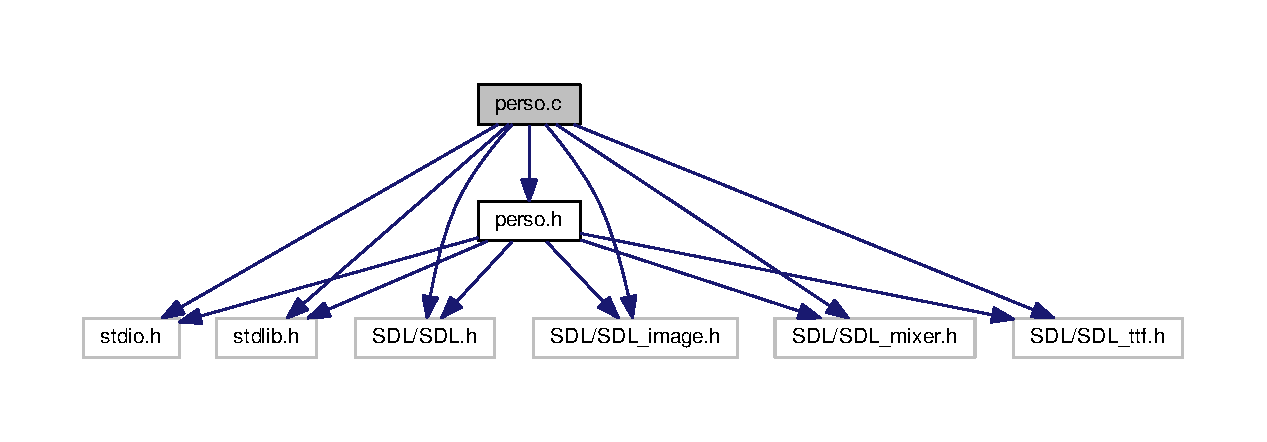
\includegraphics[width=350pt]{perso_8c__incl}
\end{center}
\end{figure}
\subsection*{Functions}
\begin{DoxyCompactItemize}
\item 
\hyperlink{structpersonnage}{personnage} \hyperlink{perso_8c_aefdd3ed151582e68d8142d416f944def}{initperso} (\hyperlink{structpersonnage}{personnage} c)
\begin{DoxyCompactList}\small\item\em to initialize hero \end{DoxyCompactList}\item 
void \hyperlink{perso_8c_a4fcd9448740c67449649edb846515fae}{affichageperso} (\hyperlink{structpersonnage}{personnage} c, S\+D\+L\+\_\+\+Surface $\ast$screen)
\begin{DoxyCompactList}\small\item\em 

 \end{DoxyCompactList}\item 
void \hyperlink{perso_8c_a176ddce8a9e039b9acad0706a7cc5d5b}{freesurfaceperso} (\hyperlink{structpersonnage}{personnage} $\ast$c)
\begin{DoxyCompactList}\small\item\em 

 \end{DoxyCompactList}\item 
void \hyperlink{perso_8c_af81b9e13ff32af2582670fdd52ced258}{animperso} (\hyperlink{structpersonnage}{personnage} $\ast$c)
\begin{DoxyCompactList}\small\item\em to animate hero \end{DoxyCompactList}\item 
void \hyperlink{perso_8c_a936a0790f87300c4d50a1fe7959875f5}{mouvement} (\hyperlink{structpersonnage}{personnage} $\ast$c)
\item 
void \hyperlink{perso_8c_a627e8dbcc77f69a29241e6dccf38d77d}{initialiser} (\hyperlink{structbackground}{background} $\ast$b)
\begin{DoxyCompactList}\small\item\em 

 \end{DoxyCompactList}\item 
void \hyperlink{perso_8c_a2e96662eb12911c08fa0bdab84e84b7f}{setup} (S\+D\+L\+\_\+\+Surface $\ast$screen, \hyperlink{structbackground}{background} $\ast$b)
\item 
void \hyperlink{perso_8c_adfeffe6a5ec91252946ce47e842d3ca7}{scrolling\+\_\+droit} (S\+D\+L\+\_\+\+Surface $\ast$screen, \hyperlink{structbackground}{background} $\ast$b, \hyperlink{structpersonnage}{personnage} $\ast$c)
\begin{DoxyCompactList}\small\item\em 

 \end{DoxyCompactList}\item 
void \hyperlink{perso_8c_aeaaf5c82548f38656077b1b49ff8bac6}{scrolling\+\_\+gauche} (S\+D\+L\+\_\+\+Surface $\ast$screen, \hyperlink{structbackground}{background} $\ast$b, \hyperlink{structpersonnage}{personnage} $\ast$c)
\begin{DoxyCompactList}\small\item\em 

 \end{DoxyCompactList}\item 
void \hyperlink{perso_8c_aa9867b2212396203068e2ed65f182bbf}{evenement} (S\+D\+L\+\_\+\+Surface $\ast$screen, \hyperlink{structbackground}{background} $\ast$b, int direction, \hyperlink{structpersonnage}{personnage} $\ast$c)
\begin{DoxyCompactList}\small\item\em 

 \end{DoxyCompactList}\end{DoxyCompactItemize}


\subsection{Detailed Description}
Bouabker Arij \begin{DoxyDate}{Date}
Mai ,2020
\end{DoxyDate}
testing program for main character animation 

\subsection{Function Documentation}
\index{perso.\+c@{perso.\+c}!affichageperso@{affichageperso}}
\index{affichageperso@{affichageperso}!perso.\+c@{perso.\+c}}
\subsubsection[{\texorpdfstring{affichageperso(personnage c, S\+D\+L\+\_\+\+Surface $\ast$screen)}{affichageperso(personnage c, SDL_Surface *screen)}}]{\setlength{\rightskip}{0pt plus 5cm}void affichageperso (
\begin{DoxyParamCaption}
\item[{{\bf personnage}}]{c, }
\item[{S\+D\+L\+\_\+\+Surface $\ast$}]{screen}
\end{DoxyParamCaption}
)}\hypertarget{perso_8c_a4fcd9448740c67449649edb846515fae}{}\label{perso_8c_a4fcd9448740c67449649edb846515fae}




 

to display hero 

Here is the call graph for this function\+:\nopagebreak
\begin{figure}[H]
\begin{center}
\leavevmode
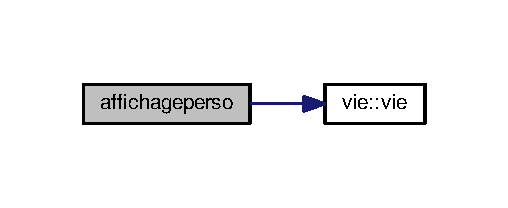
\includegraphics[width=244pt]{perso_8c_a4fcd9448740c67449649edb846515fae_cgraph}
\end{center}
\end{figure}




Here is the caller graph for this function\+:\nopagebreak
\begin{figure}[H]
\begin{center}
\leavevmode
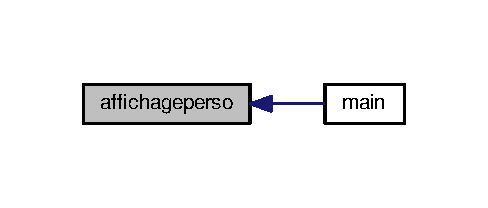
\includegraphics[width=234pt]{perso_8c_a4fcd9448740c67449649edb846515fae_icgraph}
\end{center}
\end{figure}


\index{perso.\+c@{perso.\+c}!animperso@{animperso}}
\index{animperso@{animperso}!perso.\+c@{perso.\+c}}
\subsubsection[{\texorpdfstring{animperso(personnage $\ast$c)}{animperso(personnage *c)}}]{\setlength{\rightskip}{0pt plus 5cm}void animperso (
\begin{DoxyParamCaption}
\item[{{\bf personnage} $\ast$}]{c}
\end{DoxyParamCaption}
)}\hypertarget{perso_8c_af81b9e13ff32af2582670fdd52ced258}{}\label{perso_8c_af81b9e13ff32af2582670fdd52ced258}


to animate hero 


\begin{DoxyParams}{Parameters}
{\em c=personnage} & \\
\hline
\end{DoxyParams}
\begin{DoxyReturn}{Returns}
nothing 
\end{DoxyReturn}


Here is the caller graph for this function\+:\nopagebreak
\begin{figure}[H]
\begin{center}
\leavevmode
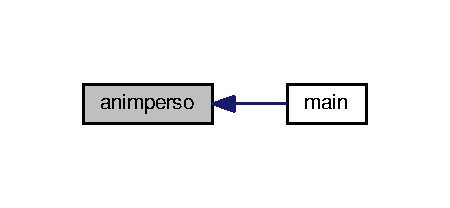
\includegraphics[width=216pt]{perso_8c_af81b9e13ff32af2582670fdd52ced258_icgraph}
\end{center}
\end{figure}


\index{perso.\+c@{perso.\+c}!evenement@{evenement}}
\index{evenement@{evenement}!perso.\+c@{perso.\+c}}
\subsubsection[{\texorpdfstring{evenement(\+S\+D\+L\+\_\+\+Surface $\ast$screen, background $\ast$b, int direction, personnage $\ast$c)}{evenement(SDL_Surface *screen, background *b, int direction, personnage *c)}}]{\setlength{\rightskip}{0pt plus 5cm}void evenement (
\begin{DoxyParamCaption}
\item[{S\+D\+L\+\_\+\+Surface $\ast$}]{screen, }
\item[{{\bf background} $\ast$}]{b, }
\item[{int}]{direction, }
\item[{{\bf personnage} $\ast$}]{c}
\end{DoxyParamCaption}
)}\hypertarget{perso_8c_aa9867b2212396203068e2ed65f182bbf}{}\label{perso_8c_aa9867b2212396203068e2ed65f182bbf}




 



Here is the call graph for this function\+:\nopagebreak
\begin{figure}[H]
\begin{center}
\leavevmode
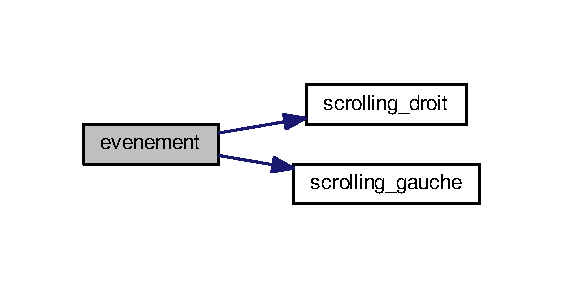
\includegraphics[width=270pt]{perso_8c_aa9867b2212396203068e2ed65f182bbf_cgraph}
\end{center}
\end{figure}




Here is the caller graph for this function\+:\nopagebreak
\begin{figure}[H]
\begin{center}
\leavevmode
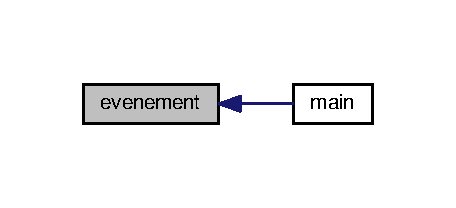
\includegraphics[width=219pt]{perso_8c_aa9867b2212396203068e2ed65f182bbf_icgraph}
\end{center}
\end{figure}


\index{perso.\+c@{perso.\+c}!freesurfaceperso@{freesurfaceperso}}
\index{freesurfaceperso@{freesurfaceperso}!perso.\+c@{perso.\+c}}
\subsubsection[{\texorpdfstring{freesurfaceperso(personnage $\ast$c)}{freesurfaceperso(personnage *c)}}]{\setlength{\rightskip}{0pt plus 5cm}void freesurfaceperso (
\begin{DoxyParamCaption}
\item[{{\bf personnage} $\ast$}]{c}
\end{DoxyParamCaption}
)}\hypertarget{perso_8c_a176ddce8a9e039b9acad0706a7cc5d5b}{}\label{perso_8c_a176ddce8a9e039b9acad0706a7cc5d5b}




 

to free memory from hero 

Here is the call graph for this function\+:\nopagebreak
\begin{figure}[H]
\begin{center}
\leavevmode
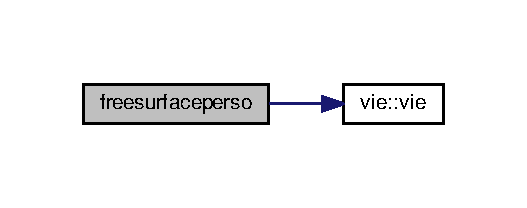
\includegraphics[width=253pt]{perso_8c_a176ddce8a9e039b9acad0706a7cc5d5b_cgraph}
\end{center}
\end{figure}


\index{perso.\+c@{perso.\+c}!initialiser@{initialiser}}
\index{initialiser@{initialiser}!perso.\+c@{perso.\+c}}
\subsubsection[{\texorpdfstring{initialiser(background $\ast$b)}{initialiser(background *b)}}]{\setlength{\rightskip}{0pt plus 5cm}void initialiser (
\begin{DoxyParamCaption}
\item[{{\bf background} $\ast$}]{b}
\end{DoxyParamCaption}
)}\hypertarget{perso_8c_a627e8dbcc77f69a29241e6dccf38d77d}{}\label{perso_8c_a627e8dbcc77f69a29241e6dccf38d77d}




 



Here is the caller graph for this function\+:\nopagebreak
\begin{figure}[H]
\begin{center}
\leavevmode
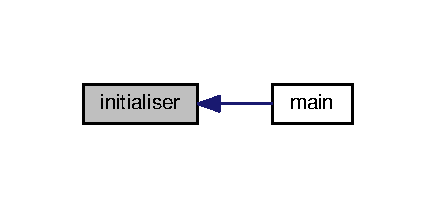
\includegraphics[width=209pt]{perso_8c_a627e8dbcc77f69a29241e6dccf38d77d_icgraph}
\end{center}
\end{figure}


\index{perso.\+c@{perso.\+c}!initperso@{initperso}}
\index{initperso@{initperso}!perso.\+c@{perso.\+c}}
\subsubsection[{\texorpdfstring{initperso(personnage c)}{initperso(personnage c)}}]{\setlength{\rightskip}{0pt plus 5cm}{\bf personnage} initperso (
\begin{DoxyParamCaption}
\item[{{\bf personnage}}]{c}
\end{DoxyParamCaption}
)}\hypertarget{perso_8c_aefdd3ed151582e68d8142d416f944def}{}\label{perso_8c_aefdd3ed151582e68d8142d416f944def}


to initialize hero 


\begin{DoxyParams}{Parameters}
{\em c=personnage} & \\
\hline
\end{DoxyParams}
\begin{DoxyReturn}{Returns}
personnage 
\end{DoxyReturn}


Here is the call graph for this function\+:\nopagebreak
\begin{figure}[H]
\begin{center}
\leavevmode
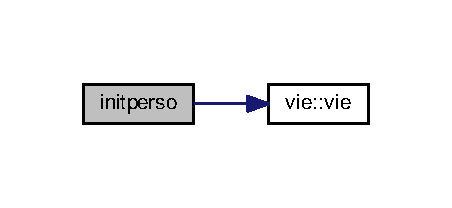
\includegraphics[width=217pt]{perso_8c_aefdd3ed151582e68d8142d416f944def_cgraph}
\end{center}
\end{figure}




Here is the caller graph for this function\+:\nopagebreak
\begin{figure}[H]
\begin{center}
\leavevmode
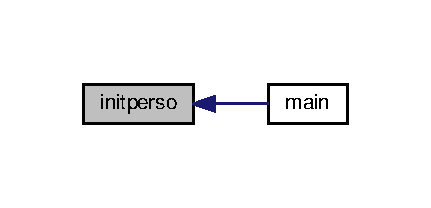
\includegraphics[width=207pt]{perso_8c_aefdd3ed151582e68d8142d416f944def_icgraph}
\end{center}
\end{figure}


\index{perso.\+c@{perso.\+c}!mouvement@{mouvement}}
\index{mouvement@{mouvement}!perso.\+c@{perso.\+c}}
\subsubsection[{\texorpdfstring{mouvement(personnage $\ast$c)}{mouvement(personnage *c)}}]{\setlength{\rightskip}{0pt plus 5cm}void mouvement (
\begin{DoxyParamCaption}
\item[{{\bf personnage} $\ast$}]{c}
\end{DoxyParamCaption}
)}\hypertarget{perso_8c_a936a0790f87300c4d50a1fe7959875f5}{}\label{perso_8c_a936a0790f87300c4d50a1fe7959875f5}


Here is the caller graph for this function\+:\nopagebreak
\begin{figure}[H]
\begin{center}
\leavevmode
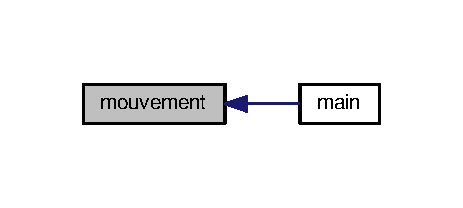
\includegraphics[width=222pt]{perso_8c_a936a0790f87300c4d50a1fe7959875f5_icgraph}
\end{center}
\end{figure}


\index{perso.\+c@{perso.\+c}!scrolling\+\_\+droit@{scrolling\+\_\+droit}}
\index{scrolling\+\_\+droit@{scrolling\+\_\+droit}!perso.\+c@{perso.\+c}}
\subsubsection[{\texorpdfstring{scrolling\+\_\+droit(\+S\+D\+L\+\_\+\+Surface $\ast$screen, background $\ast$b, personnage $\ast$c)}{scrolling_droit(SDL_Surface *screen, background *b, personnage *c)}}]{\setlength{\rightskip}{0pt plus 5cm}void scrolling\+\_\+droit (
\begin{DoxyParamCaption}
\item[{S\+D\+L\+\_\+\+Surface $\ast$}]{screen, }
\item[{{\bf background} $\ast$}]{b, }
\item[{{\bf personnage} $\ast$}]{c}
\end{DoxyParamCaption}
)}\hypertarget{perso_8c_adfeffe6a5ec91252946ce47e842d3ca7}{}\label{perso_8c_adfeffe6a5ec91252946ce47e842d3ca7}




 



Here is the caller graph for this function\+:\nopagebreak
\begin{figure}[H]
\begin{center}
\leavevmode
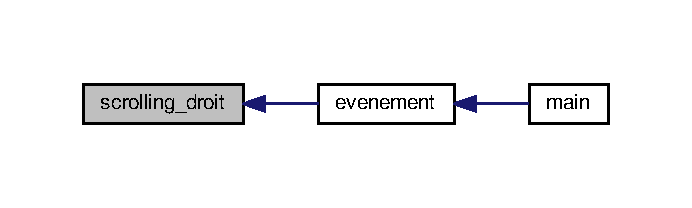
\includegraphics[width=332pt]{perso_8c_adfeffe6a5ec91252946ce47e842d3ca7_icgraph}
\end{center}
\end{figure}


\index{perso.\+c@{perso.\+c}!scrolling\+\_\+gauche@{scrolling\+\_\+gauche}}
\index{scrolling\+\_\+gauche@{scrolling\+\_\+gauche}!perso.\+c@{perso.\+c}}
\subsubsection[{\texorpdfstring{scrolling\+\_\+gauche(\+S\+D\+L\+\_\+\+Surface $\ast$screen, background $\ast$b, personnage $\ast$c)}{scrolling_gauche(SDL_Surface *screen, background *b, personnage *c)}}]{\setlength{\rightskip}{0pt plus 5cm}void scrolling\+\_\+gauche (
\begin{DoxyParamCaption}
\item[{S\+D\+L\+\_\+\+Surface $\ast$}]{screen, }
\item[{{\bf background} $\ast$}]{b, }
\item[{{\bf personnage} $\ast$}]{c}
\end{DoxyParamCaption}
)}\hypertarget{perso_8c_aeaaf5c82548f38656077b1b49ff8bac6}{}\label{perso_8c_aeaaf5c82548f38656077b1b49ff8bac6}




 



Here is the caller graph for this function\+:\nopagebreak
\begin{figure}[H]
\begin{center}
\leavevmode
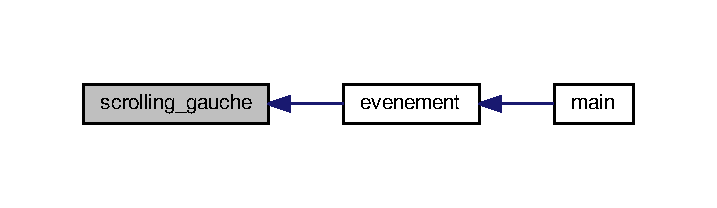
\includegraphics[width=344pt]{perso_8c_aeaaf5c82548f38656077b1b49ff8bac6_icgraph}
\end{center}
\end{figure}


\index{perso.\+c@{perso.\+c}!setup@{setup}}
\index{setup@{setup}!perso.\+c@{perso.\+c}}
\subsubsection[{\texorpdfstring{setup(\+S\+D\+L\+\_\+\+Surface $\ast$screen, background $\ast$b)}{setup(SDL_Surface *screen, background *b)}}]{\setlength{\rightskip}{0pt plus 5cm}void setup (
\begin{DoxyParamCaption}
\item[{S\+D\+L\+\_\+\+Surface $\ast$}]{screen, }
\item[{{\bf background} $\ast$}]{b}
\end{DoxyParamCaption}
)}\hypertarget{perso_8c_a2e96662eb12911c08fa0bdab84e84b7f}{}\label{perso_8c_a2e96662eb12911c08fa0bdab84e84b7f}


Here is the caller graph for this function\+:\nopagebreak
\begin{figure}[H]
\begin{center}
\leavevmode
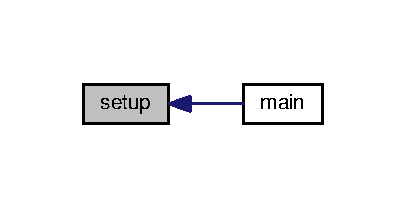
\includegraphics[width=195pt]{perso_8c_a2e96662eb12911c08fa0bdab84e84b7f_icgraph}
\end{center}
\end{figure}



\hypertarget{perso_8h}{}\section{perso.\+h File Reference}
\label{perso_8h}\index{perso.\+h@{perso.\+h}}
{\ttfamily \#include $<$stdio.\+h$>$}\\*
{\ttfamily \#include $<$stdlib.\+h$>$}\\*
{\ttfamily \#include \char`\"{}S\+D\+L/\+S\+D\+L.\+h\char`\"{}}\\*
{\ttfamily \#include \char`\"{}S\+D\+L/\+S\+D\+L\+\_\+image.\+h\char`\"{}}\\*
{\ttfamily \#include \char`\"{}S\+D\+L/\+S\+D\+L\+\_\+mixer.\+h\char`\"{}}\\*
{\ttfamily \#include \char`\"{}S\+D\+L/\+S\+D\+L\+\_\+ttf.\+h\char`\"{}}\\*
Include dependency graph for perso.\+h\+:\nopagebreak
\begin{figure}[H]
\begin{center}
\leavevmode
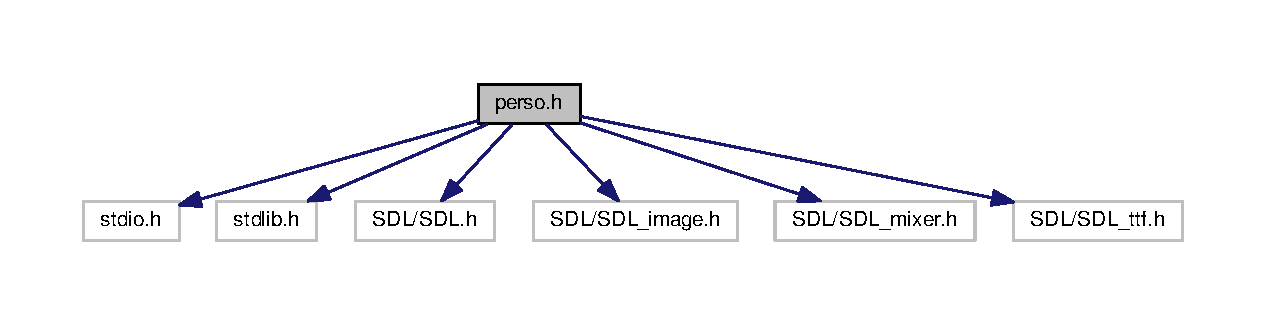
\includegraphics[width=350pt]{perso_8h__incl}
\end{center}
\end{figure}
This graph shows which files directly or indirectly include this file\+:\nopagebreak
\begin{figure}[H]
\begin{center}
\leavevmode
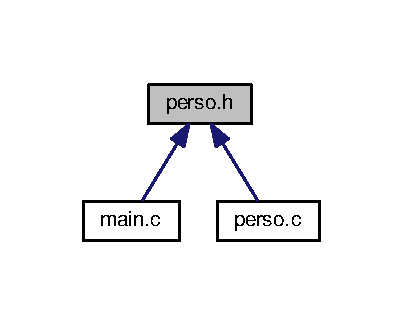
\includegraphics[width=194pt]{perso_8h__dep__incl}
\end{center}
\end{figure}
\subsection*{Classes}
\begin{DoxyCompactItemize}
\item 
struct \hyperlink{structbackground}{background}
\begin{DoxyCompactList}\small\item\em struct for background \end{DoxyCompactList}\item 
struct \hyperlink{structvie}{vie}
\begin{DoxyCompactList}\small\item\em struct for life of hero \end{DoxyCompactList}\item 
struct \hyperlink{structscore}{score}
\begin{DoxyCompactList}\small\item\em struct for score of hero \end{DoxyCompactList}\item 
struct \hyperlink{structpersonnage}{personnage}
\begin{DoxyCompactList}\small\item\em struct for hero \end{DoxyCompactList}\end{DoxyCompactItemize}
\subsection*{Macros}
\begin{DoxyCompactItemize}
\item 
\#define \hyperlink{perso_8h_a09f1cd4ab0356c6e8f1fae7ad5b5e1b7}{mapw}~6838
\item 
\#define \hyperlink{perso_8h_afc4a978b3c563d99156af79d4312b602}{maph}~613
\item 
\#define \hyperlink{perso_8h_a256fa45915e06d853830477e42cea383}{hero\+\_\+sprite\+\_\+W}~200
\item 
\#define \hyperlink{perso_8h_aa9d0b49e693cbe649a0dd7f6e9a5f37b}{hero\+\_\+sprite\+\_\+H}~300
\end{DoxyCompactItemize}
\subsection*{Typedefs}
\begin{DoxyCompactItemize}
\item 
typedef struct \hyperlink{structvie}{vie} \hyperlink{perso_8h_a5a50eadb578d4b4b9db54fdffc9b3c48}{vie}
\item 
typedef struct \hyperlink{structscore}{score} \hyperlink{perso_8h_a1240ca29fa6f99334b17271ea026bc91}{score}
\item 
typedef struct \hyperlink{structpersonnage}{personnage} \hyperlink{perso_8h_a22ea6c21be7b6540d95f47b6ad40ffa6}{personnage}
\end{DoxyCompactItemize}
\subsection*{Functions}
\begin{DoxyCompactItemize}
\item 
\hyperlink{structpersonnage}{personnage} \hyperlink{perso_8h_aefdd3ed151582e68d8142d416f944def}{initperso} (\hyperlink{structpersonnage}{personnage} c)
\begin{DoxyCompactList}\small\item\em to initialize hero \end{DoxyCompactList}\item 
void \hyperlink{perso_8h_a4fcd9448740c67449649edb846515fae}{affichageperso} (\hyperlink{structpersonnage}{personnage} c, S\+D\+L\+\_\+\+Surface $\ast$screen)
\begin{DoxyCompactList}\small\item\em to display hero \end{DoxyCompactList}\item 
void \hyperlink{perso_8h_af81b9e13ff32af2582670fdd52ced258}{animperso} (\hyperlink{structpersonnage}{personnage} $\ast$c)
\begin{DoxyCompactList}\small\item\em to animate hero \end{DoxyCompactList}\item 
void \hyperlink{perso_8h_a176ddce8a9e039b9acad0706a7cc5d5b}{freesurfaceperso} (\hyperlink{structpersonnage}{personnage} $\ast$c)
\begin{DoxyCompactList}\small\item\em to free memory from hero \end{DoxyCompactList}\item 
void \hyperlink{perso_8h_a936a0790f87300c4d50a1fe7959875f5}{mouvement} (\hyperlink{structpersonnage}{personnage} $\ast$c)
\item 
void \hyperlink{perso_8h_a627e8dbcc77f69a29241e6dccf38d77d}{initialiser} (\hyperlink{structbackground}{background} $\ast$b)
\begin{DoxyCompactList}\small\item\em 

 \end{DoxyCompactList}\item 
void \hyperlink{perso_8h_aeaaf5c82548f38656077b1b49ff8bac6}{scrolling\+\_\+gauche} (S\+D\+L\+\_\+\+Surface $\ast$screen, \hyperlink{structbackground}{background} $\ast$b, \hyperlink{structpersonnage}{personnage} $\ast$c)
\begin{DoxyCompactList}\small\item\em 

 \end{DoxyCompactList}\item 
void \hyperlink{perso_8h_aa9867b2212396203068e2ed65f182bbf}{evenement} (S\+D\+L\+\_\+\+Surface $\ast$screen, \hyperlink{structbackground}{background} $\ast$b, int direction, \hyperlink{structpersonnage}{personnage} $\ast$c)
\begin{DoxyCompactList}\small\item\em 

 \end{DoxyCompactList}\item 
void \hyperlink{perso_8h_adfeffe6a5ec91252946ce47e842d3ca7}{scrolling\+\_\+droit} (S\+D\+L\+\_\+\+Surface $\ast$screen, \hyperlink{structbackground}{background} $\ast$b, \hyperlink{structpersonnage}{personnage} $\ast$c)
\begin{DoxyCompactList}\small\item\em 

 \end{DoxyCompactList}\item 
void \hyperlink{perso_8h_a2e96662eb12911c08fa0bdab84e84b7f}{setup} (S\+D\+L\+\_\+\+Surface $\ast$screen, \hyperlink{structbackground}{background} $\ast$b)
\end{DoxyCompactItemize}


\subsection{Detailed Description}
Bouabker Arij \begin{DoxyDate}{Date}
Mai ,2020
\end{DoxyDate}
testing program for main character animation 

\subsection{Macro Definition Documentation}
\index{perso.\+h@{perso.\+h}!hero\+\_\+sprite\+\_\+H@{hero\+\_\+sprite\+\_\+H}}
\index{hero\+\_\+sprite\+\_\+H@{hero\+\_\+sprite\+\_\+H}!perso.\+h@{perso.\+h}}
\subsubsection[{\texorpdfstring{hero\+\_\+sprite\+\_\+H}{hero_sprite_H}}]{\setlength{\rightskip}{0pt plus 5cm}\#define hero\+\_\+sprite\+\_\+H~300}\hypertarget{perso_8h_aa9d0b49e693cbe649a0dd7f6e9a5f37b}{}\label{perso_8h_aa9d0b49e693cbe649a0dd7f6e9a5f37b}
\index{perso.\+h@{perso.\+h}!hero\+\_\+sprite\+\_\+W@{hero\+\_\+sprite\+\_\+W}}
\index{hero\+\_\+sprite\+\_\+W@{hero\+\_\+sprite\+\_\+W}!perso.\+h@{perso.\+h}}
\subsubsection[{\texorpdfstring{hero\+\_\+sprite\+\_\+W}{hero_sprite_W}}]{\setlength{\rightskip}{0pt plus 5cm}\#define hero\+\_\+sprite\+\_\+W~200}\hypertarget{perso_8h_a256fa45915e06d853830477e42cea383}{}\label{perso_8h_a256fa45915e06d853830477e42cea383}
\index{perso.\+h@{perso.\+h}!maph@{maph}}
\index{maph@{maph}!perso.\+h@{perso.\+h}}
\subsubsection[{\texorpdfstring{maph}{maph}}]{\setlength{\rightskip}{0pt plus 5cm}\#define maph~613}\hypertarget{perso_8h_afc4a978b3c563d99156af79d4312b602}{}\label{perso_8h_afc4a978b3c563d99156af79d4312b602}
\index{perso.\+h@{perso.\+h}!mapw@{mapw}}
\index{mapw@{mapw}!perso.\+h@{perso.\+h}}
\subsubsection[{\texorpdfstring{mapw}{mapw}}]{\setlength{\rightskip}{0pt plus 5cm}\#define mapw~6838}\hypertarget{perso_8h_a09f1cd4ab0356c6e8f1fae7ad5b5e1b7}{}\label{perso_8h_a09f1cd4ab0356c6e8f1fae7ad5b5e1b7}


\subsection{Typedef Documentation}
\index{perso.\+h@{perso.\+h}!personnage@{personnage}}
\index{personnage@{personnage}!perso.\+h@{perso.\+h}}
\subsubsection[{\texorpdfstring{personnage}{personnage}}]{\setlength{\rightskip}{0pt plus 5cm}typedef struct {\bf personnage}  {\bf personnage}}\hypertarget{perso_8h_a22ea6c21be7b6540d95f47b6ad40ffa6}{}\label{perso_8h_a22ea6c21be7b6540d95f47b6ad40ffa6}
\index{perso.\+h@{perso.\+h}!score@{score}}
\index{score@{score}!perso.\+h@{perso.\+h}}
\subsubsection[{\texorpdfstring{score}{score}}]{\setlength{\rightskip}{0pt plus 5cm}typedef struct {\bf score} {\bf score}}\hypertarget{perso_8h_a1240ca29fa6f99334b17271ea026bc91}{}\label{perso_8h_a1240ca29fa6f99334b17271ea026bc91}
\index{perso.\+h@{perso.\+h}!vie@{vie}}
\index{vie@{vie}!perso.\+h@{perso.\+h}}
\subsubsection[{\texorpdfstring{vie}{vie}}]{\setlength{\rightskip}{0pt plus 5cm}typedef struct {\bf vie} {\bf vie}}\hypertarget{perso_8h_a5a50eadb578d4b4b9db54fdffc9b3c48}{}\label{perso_8h_a5a50eadb578d4b4b9db54fdffc9b3c48}


\subsection{Function Documentation}
\index{perso.\+h@{perso.\+h}!affichageperso@{affichageperso}}
\index{affichageperso@{affichageperso}!perso.\+h@{perso.\+h}}
\subsubsection[{\texorpdfstring{affichageperso(personnage c, S\+D\+L\+\_\+\+Surface $\ast$screen)}{affichageperso(personnage c, SDL_Surface *screen)}}]{\setlength{\rightskip}{0pt plus 5cm}void affichageperso (
\begin{DoxyParamCaption}
\item[{{\bf personnage}}]{c, }
\item[{S\+D\+L\+\_\+\+Surface $\ast$}]{screen}
\end{DoxyParamCaption}
)}\hypertarget{perso_8h_a4fcd9448740c67449649edb846515fae}{}\label{perso_8h_a4fcd9448740c67449649edb846515fae}


to display hero 


\begin{DoxyParams}{Parameters}
{\em c=personnage} & \\
\hline
{\em screen} & the screen \\
\hline
\end{DoxyParams}
\begin{DoxyReturn}{Returns}
nothing
\end{DoxyReturn}
to display hero 

Here is the call graph for this function\+:\nopagebreak
\begin{figure}[H]
\begin{center}
\leavevmode
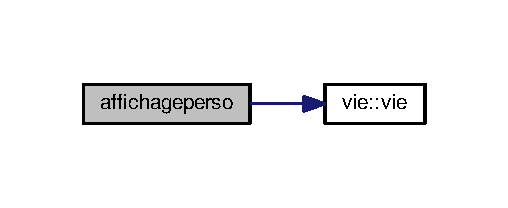
\includegraphics[width=244pt]{perso_8h_a4fcd9448740c67449649edb846515fae_cgraph}
\end{center}
\end{figure}




Here is the caller graph for this function\+:\nopagebreak
\begin{figure}[H]
\begin{center}
\leavevmode
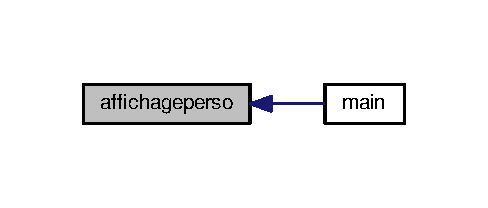
\includegraphics[width=234pt]{perso_8h_a4fcd9448740c67449649edb846515fae_icgraph}
\end{center}
\end{figure}


\index{perso.\+h@{perso.\+h}!animperso@{animperso}}
\index{animperso@{animperso}!perso.\+h@{perso.\+h}}
\subsubsection[{\texorpdfstring{animperso(personnage $\ast$c)}{animperso(personnage *c)}}]{\setlength{\rightskip}{0pt plus 5cm}void animperso (
\begin{DoxyParamCaption}
\item[{{\bf personnage} $\ast$}]{c}
\end{DoxyParamCaption}
)}\hypertarget{perso_8h_af81b9e13ff32af2582670fdd52ced258}{}\label{perso_8h_af81b9e13ff32af2582670fdd52ced258}


to animate hero 


\begin{DoxyParams}{Parameters}
{\em c=personnage} & \\
\hline
\end{DoxyParams}
\begin{DoxyReturn}{Returns}
nothing 
\end{DoxyReturn}


Here is the caller graph for this function\+:\nopagebreak
\begin{figure}[H]
\begin{center}
\leavevmode
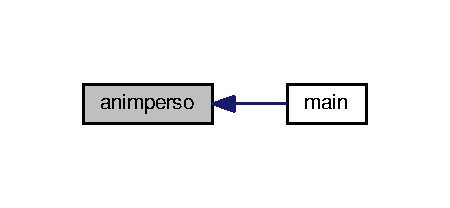
\includegraphics[width=216pt]{perso_8h_af81b9e13ff32af2582670fdd52ced258_icgraph}
\end{center}
\end{figure}


\index{perso.\+h@{perso.\+h}!evenement@{evenement}}
\index{evenement@{evenement}!perso.\+h@{perso.\+h}}
\subsubsection[{\texorpdfstring{evenement(\+S\+D\+L\+\_\+\+Surface $\ast$screen, background $\ast$b, int direction, personnage $\ast$c)}{evenement(SDL_Surface *screen, background *b, int direction, personnage *c)}}]{\setlength{\rightskip}{0pt plus 5cm}void evenement (
\begin{DoxyParamCaption}
\item[{S\+D\+L\+\_\+\+Surface $\ast$}]{screen, }
\item[{{\bf background} $\ast$}]{b, }
\item[{int}]{direction, }
\item[{{\bf personnage} $\ast$}]{c}
\end{DoxyParamCaption}
)}\hypertarget{perso_8h_aa9867b2212396203068e2ed65f182bbf}{}\label{perso_8h_aa9867b2212396203068e2ed65f182bbf}




 



Here is the call graph for this function\+:\nopagebreak
\begin{figure}[H]
\begin{center}
\leavevmode
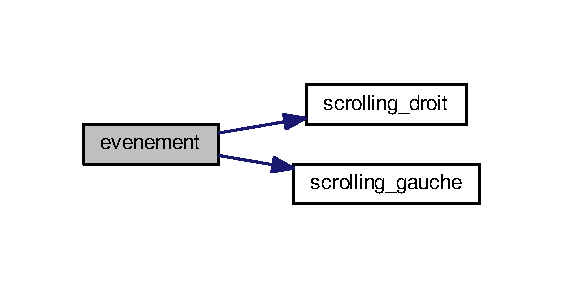
\includegraphics[width=270pt]{perso_8h_aa9867b2212396203068e2ed65f182bbf_cgraph}
\end{center}
\end{figure}




Here is the caller graph for this function\+:\nopagebreak
\begin{figure}[H]
\begin{center}
\leavevmode
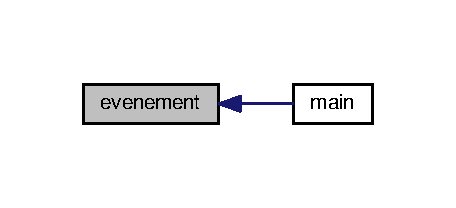
\includegraphics[width=219pt]{perso_8h_aa9867b2212396203068e2ed65f182bbf_icgraph}
\end{center}
\end{figure}


\index{perso.\+h@{perso.\+h}!freesurfaceperso@{freesurfaceperso}}
\index{freesurfaceperso@{freesurfaceperso}!perso.\+h@{perso.\+h}}
\subsubsection[{\texorpdfstring{freesurfaceperso(personnage $\ast$c)}{freesurfaceperso(personnage *c)}}]{\setlength{\rightskip}{0pt plus 5cm}void freesurfaceperso (
\begin{DoxyParamCaption}
\item[{{\bf personnage} $\ast$}]{c}
\end{DoxyParamCaption}
)}\hypertarget{perso_8h_a176ddce8a9e039b9acad0706a7cc5d5b}{}\label{perso_8h_a176ddce8a9e039b9acad0706a7cc5d5b}


to free memory from hero 


\begin{DoxyParams}{Parameters}
{\em c=personnage} & \\
\hline
\end{DoxyParams}
\begin{DoxyReturn}{Returns}
nothing
\end{DoxyReturn}
to free memory from hero 

Here is the call graph for this function\+:\nopagebreak
\begin{figure}[H]
\begin{center}
\leavevmode
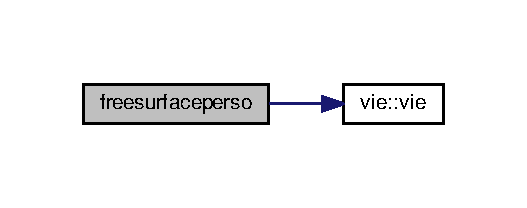
\includegraphics[width=253pt]{perso_8h_a176ddce8a9e039b9acad0706a7cc5d5b_cgraph}
\end{center}
\end{figure}


\index{perso.\+h@{perso.\+h}!initialiser@{initialiser}}
\index{initialiser@{initialiser}!perso.\+h@{perso.\+h}}
\subsubsection[{\texorpdfstring{initialiser(background $\ast$b)}{initialiser(background *b)}}]{\setlength{\rightskip}{0pt plus 5cm}void initialiser (
\begin{DoxyParamCaption}
\item[{{\bf background} $\ast$}]{b}
\end{DoxyParamCaption}
)}\hypertarget{perso_8h_a627e8dbcc77f69a29241e6dccf38d77d}{}\label{perso_8h_a627e8dbcc77f69a29241e6dccf38d77d}




 



Here is the caller graph for this function\+:\nopagebreak
\begin{figure}[H]
\begin{center}
\leavevmode
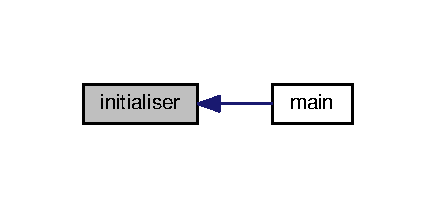
\includegraphics[width=209pt]{perso_8h_a627e8dbcc77f69a29241e6dccf38d77d_icgraph}
\end{center}
\end{figure}


\index{perso.\+h@{perso.\+h}!initperso@{initperso}}
\index{initperso@{initperso}!perso.\+h@{perso.\+h}}
\subsubsection[{\texorpdfstring{initperso(personnage c)}{initperso(personnage c)}}]{\setlength{\rightskip}{0pt plus 5cm}{\bf personnage} initperso (
\begin{DoxyParamCaption}
\item[{{\bf personnage}}]{c}
\end{DoxyParamCaption}
)}\hypertarget{perso_8h_aefdd3ed151582e68d8142d416f944def}{}\label{perso_8h_aefdd3ed151582e68d8142d416f944def}


to initialize hero 


\begin{DoxyParams}{Parameters}
{\em c=personnage} & \\
\hline
\end{DoxyParams}
\begin{DoxyReturn}{Returns}
personnage 
\end{DoxyReturn}


Here is the call graph for this function\+:\nopagebreak
\begin{figure}[H]
\begin{center}
\leavevmode
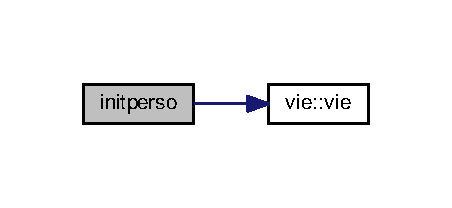
\includegraphics[width=217pt]{perso_8h_aefdd3ed151582e68d8142d416f944def_cgraph}
\end{center}
\end{figure}




Here is the caller graph for this function\+:\nopagebreak
\begin{figure}[H]
\begin{center}
\leavevmode
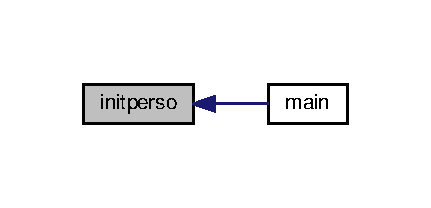
\includegraphics[width=207pt]{perso_8h_aefdd3ed151582e68d8142d416f944def_icgraph}
\end{center}
\end{figure}


\index{perso.\+h@{perso.\+h}!mouvement@{mouvement}}
\index{mouvement@{mouvement}!perso.\+h@{perso.\+h}}
\subsubsection[{\texorpdfstring{mouvement(personnage $\ast$c)}{mouvement(personnage *c)}}]{\setlength{\rightskip}{0pt plus 5cm}void mouvement (
\begin{DoxyParamCaption}
\item[{{\bf personnage} $\ast$}]{c}
\end{DoxyParamCaption}
)}\hypertarget{perso_8h_a936a0790f87300c4d50a1fe7959875f5}{}\label{perso_8h_a936a0790f87300c4d50a1fe7959875f5}


Here is the caller graph for this function\+:\nopagebreak
\begin{figure}[H]
\begin{center}
\leavevmode
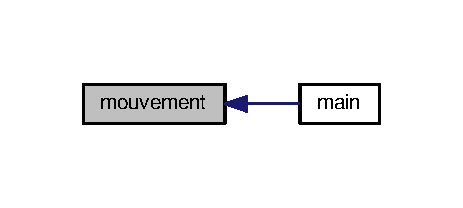
\includegraphics[width=222pt]{perso_8h_a936a0790f87300c4d50a1fe7959875f5_icgraph}
\end{center}
\end{figure}


\index{perso.\+h@{perso.\+h}!scrolling\+\_\+droit@{scrolling\+\_\+droit}}
\index{scrolling\+\_\+droit@{scrolling\+\_\+droit}!perso.\+h@{perso.\+h}}
\subsubsection[{\texorpdfstring{scrolling\+\_\+droit(\+S\+D\+L\+\_\+\+Surface $\ast$screen, background $\ast$b, personnage $\ast$c)}{scrolling_droit(SDL_Surface *screen, background *b, personnage *c)}}]{\setlength{\rightskip}{0pt plus 5cm}void scrolling\+\_\+droit (
\begin{DoxyParamCaption}
\item[{S\+D\+L\+\_\+\+Surface $\ast$}]{screen, }
\item[{{\bf background} $\ast$}]{b, }
\item[{{\bf personnage} $\ast$}]{c}
\end{DoxyParamCaption}
)}\hypertarget{perso_8h_adfeffe6a5ec91252946ce47e842d3ca7}{}\label{perso_8h_adfeffe6a5ec91252946ce47e842d3ca7}




 



Here is the caller graph for this function\+:\nopagebreak
\begin{figure}[H]
\begin{center}
\leavevmode
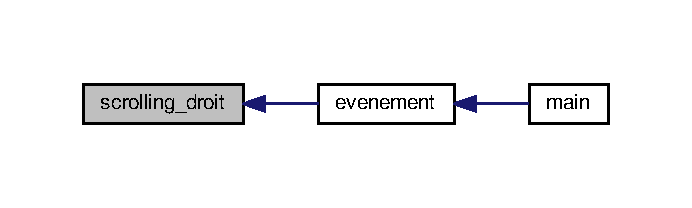
\includegraphics[width=332pt]{perso_8h_adfeffe6a5ec91252946ce47e842d3ca7_icgraph}
\end{center}
\end{figure}


\index{perso.\+h@{perso.\+h}!scrolling\+\_\+gauche@{scrolling\+\_\+gauche}}
\index{scrolling\+\_\+gauche@{scrolling\+\_\+gauche}!perso.\+h@{perso.\+h}}
\subsubsection[{\texorpdfstring{scrolling\+\_\+gauche(\+S\+D\+L\+\_\+\+Surface $\ast$screen, background $\ast$b, personnage $\ast$c)}{scrolling_gauche(SDL_Surface *screen, background *b, personnage *c)}}]{\setlength{\rightskip}{0pt plus 5cm}void scrolling\+\_\+gauche (
\begin{DoxyParamCaption}
\item[{S\+D\+L\+\_\+\+Surface $\ast$}]{screen, }
\item[{{\bf background} $\ast$}]{b, }
\item[{{\bf personnage} $\ast$}]{c}
\end{DoxyParamCaption}
)}\hypertarget{perso_8h_aeaaf5c82548f38656077b1b49ff8bac6}{}\label{perso_8h_aeaaf5c82548f38656077b1b49ff8bac6}




 



Here is the caller graph for this function\+:\nopagebreak
\begin{figure}[H]
\begin{center}
\leavevmode
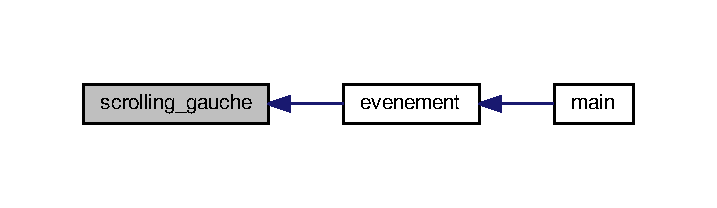
\includegraphics[width=344pt]{perso_8h_aeaaf5c82548f38656077b1b49ff8bac6_icgraph}
\end{center}
\end{figure}


\index{perso.\+h@{perso.\+h}!setup@{setup}}
\index{setup@{setup}!perso.\+h@{perso.\+h}}
\subsubsection[{\texorpdfstring{setup(\+S\+D\+L\+\_\+\+Surface $\ast$screen, background $\ast$b)}{setup(SDL_Surface *screen, background *b)}}]{\setlength{\rightskip}{0pt plus 5cm}void setup (
\begin{DoxyParamCaption}
\item[{S\+D\+L\+\_\+\+Surface $\ast$}]{screen, }
\item[{{\bf background} $\ast$}]{b}
\end{DoxyParamCaption}
)}\hypertarget{perso_8h_a2e96662eb12911c08fa0bdab84e84b7f}{}\label{perso_8h_a2e96662eb12911c08fa0bdab84e84b7f}


Here is the caller graph for this function\+:\nopagebreak
\begin{figure}[H]
\begin{center}
\leavevmode
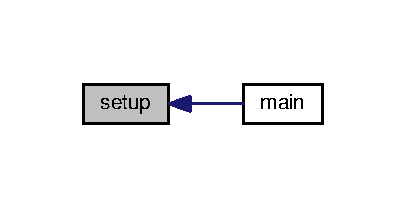
\includegraphics[width=195pt]{perso_8h_a2e96662eb12911c08fa0bdab84e84b7f_icgraph}
\end{center}
\end{figure}



%--- End generated contents ---

% Index
\backmatter
\newpage
\phantomsection
\clearemptydoublepage
\addcontentsline{toc}{chapter}{Index}
\printindex

\end{document}
